\documentclass{article}
\usepackage[brazil]{babel}
\usepackage[utf8]{inputenc}
\usepackage{amsmath}
\usepackage{Sweave} % O arquivo Sweave.sty deve estar presente

\begin{document}

\section{Um documento em Markdown}

\subsection{Sobre o Markdown}

O Markdown é uma linguagem de marcação muito simples, desenvolvida por
John Gruber.

A ideia básica por trás da linguagem é fazer com que o escritor se
preocupe mais com o \textbf{conteúdo} do texto do que com a
\emph{formatação}.

\subsection{Mais um título}

Aqui vamos tentar descrever uma análise.

\subsection{Simulando variáveis aleatórias}

No R podemos simular valores de uma distribuição normal padrão através
da função \texttt{rnorm()}.

Seja $X \sim \text{N}(0,1)$, então para gerar 30 valores dessa
variável aleatório normal, fazemos

\begin{Schunk}
\begin{Sinput}
> (x <- rnorm(30))
\end{Sinput}
\begin{Soutput}
 [1] -0.375493601 -0.604557175 -1.948110290 -0.330651659  0.828225415
 [6]  0.150294511  1.050408155  0.545060471  0.181338377 -0.586312206
[11]  1.160011828  0.228437276 -0.596343324  1.483704501 -0.327454693
[16] -1.686400728  0.005408232 -0.354338592 -0.657116839  1.077212261
[21] -0.262268573  0.858294728  0.363021095 -0.711483531 -0.913594885
[26] -1.873091184  0.322598238  0.844877539 -1.105913024  0.891034370
\end{Soutput}
\end{Schunk}

\subsection{Comentários}

Com o resultado dessa simulação, podemos calcular a média e a variância
dessa VA $X$ para conferir se o resultado fica próximo de 0 e 1,
respectivamente.

\subsection{Visualização}

Também podemos fazer um histograma dessa VA $X$ simulada

\begin{figure}
\begin{Schunk}
\begin{Sinput}
> hist(x)
\end{Sinput}
\end{Schunk}
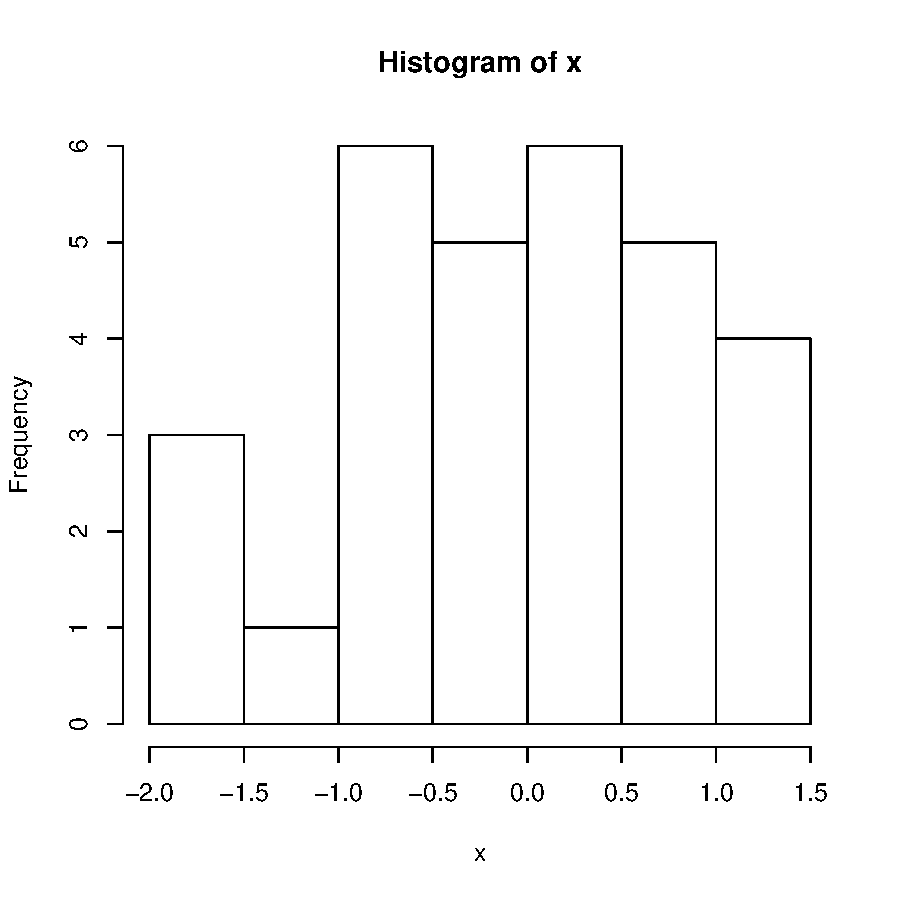
\includegraphics{Exemplo0-Sweave-histm}
\end{figure}


\end{document}
